\documentclass{book}

\usepackage{amssymb}
\usepackage{amsmath}
\usepackage{amsthm}
\usepackage{arydshln}
\usepackage{calc}
\usepackage{cancel}
\usepackage{caption}
\usepackage{cite}
\usepackage{color}
\usepackage{enumitem}
\usepackage{esint}
\usepackage{etoolbox}
\usepackage{float}
\usepackage{framed}
\usepackage{fullpage}
\usepackage{gensymb}
\usepackage[margin=1in]{geometry}
\usepackage{graphicx}
\usepackage{listings}
\usepackage{multirow}
\usepackage{subfiles}
\usepackage{rsfso}
\usepackage{tikz}
\usepackage{tikz-3dplot}
\usepackage{ushort}
\usepackage{wrapfig}
\usepackage{xcolor}
\usepackage{soul}
\usepackage{epstopdf}

% pdf versions
\pdfoptionpdfminorversion=7

% handle page stretching
\raggedbottom

% Graphics file location
\graphicspath{{Graphics/}{../Graphics/}}

% Use for drawings
\usetikzlibrary{angles,arrows,calc,decorations,intersections,patterns,positioning,quotes,shapes}
\usetikzlibrary{shapes.geometric}
\usetikzlibrary{decorations.pathreplacing}
\newcommand{\midarrow}{\tikz \draw[-latex] (0,0) -- +(.1,0);}

% Tikz commands for drawing block diagrams, etc...
\tikzset{%
	block/.style    = {draw, rectangle, minimum height = 2em, minimum width = 2em},
	sum/.style      = {draw, circle}, % Adder
	input/.style    = {fill=white, rectangle}, % Input
	output/.style   = {fill=white, rectangle}, % Output
	waypoint/.style   = {coordinate}, % Output
}

\tikzset{%
	startstop/.style= {draw, rectangle, rounded corners, minimum width=2cm, minimum height=1cm,text centered},
	inout/.style    = {draw, trapezium, trapezium left angle=70, trapezium right angle=110, minimum width=2cm, minimum height=1cm, text centered},
	process/.style  = {draw, rectangle, minimum width=2cm, minimum height=1cm, text centered},
	decision/.style = {draw, diamond, minimum width=1.5cm, minimum height=1cm, text centered, diamond, aspect=2},
	arrow/.style    = {thick,-latex,>=stealth},		
}

\tikzset{
	saveuse path/.code 2 args={
		\pgfkeysalso{#1/.style={insert path={#2}}}%
		\global\expandafter\let\csname pgfk@\pgfkeyscurrentpath/.@cmd\expandafter\endcsname
		% not optimal as it is now global through out the document
		\csname pgfk@\pgfkeyscurrentpath/.@cmd\endcsname
		\pgfkeysalso{#1}},
	/pgf/math set seed/.code=\pgfmathsetseed{#1}}

% Define Laplace, Fourier transform symbols
\newcommand{\LT}{\mathcal{L}}
\newcommand{\FT}{\mathcal{F}}

% Define adjugate function
\newcommand{\adj}{\text{adj}}

% Define rank function
\newcommand{\rank}{\text{rank}}

% commands to speed up writing j\omega and s-plane
\newcommand{\jw}{j\omega}
\newcommand{\spl}{s\textrm{-plane}}
\newcommand{\wt}{\omega t}
\newcommand{\Lm}{\textrm{Lm }}
% Clean up overline/underline for math mode
\def\obar#1{\bar{#1}}
\def\ubar#1{\ushort{#1}}

\newcommand{\exmp}{\subsubsection*{Example}}
\newcommand{\nib}{\noindent$ \bullet\ $}


\begin{document}
\chapter*{Lecture 14}
\section*{Bode diagrams for more complex systems}
We know how to sketch Bode diagrams for simple systems like $ s $, $ 1/s $, $ \tau s+1 $, and so on. If $ G(s) $ is more complex, what do we do?

Imagine factoring $ G(s) $ as:
\[ G(s) = KG_1(s)G_2(s)\ldots G_N(s) \]
where each factored term ($ G_i(s) $) is something we know how to sketch. Then in polar form we have:
\[ G(\jw) = Me^{j\phi} = K M_1e^{j\phi_1} M_2e^{j\phi_2} \ldots M_Ne^{j\phi_N} \]
\[ G(\jw) = (KM_1M_2\ldots M_N)e^{j(\phi_1+\phi_2+\ldots+\phi_N)} \]
So,
\[ M = KM_1M_2\ldots M_N \Rightarrow \Lm M = \Lm K + \Lm M_1 + \Lm M_2 + \ldots \Lm M_N \]
\[ \phi = \phi_1+\phi_2+\ldots+\phi_N \]
We can use superposition for $ \Lm M $ and $ \phi $ --- adding and together the effects of the different terms.

For superposition, we need to use a change mentality. For example:
\begin{itemize}
	\item \textbf{Don't think:} 
	\begin{itemize}
		\item $ \Lm(\tau s+1) $ is a horizontal line at 0dB for $ \omega < 1/\tau $
		\item $ \Lm(\tau s+1) $ is a line with 20dB/decade slope for $ \omega > 1/\tau $.
	\end{itemize}
	\item \textbf{Instead, think:}
	\begin{itemize}
		\item $ \Lm(\tau s+1) $ adds nothing for $ \omega < 1/\tau $
		\item $ \Lm(\tau s+1) $ adds 20dB/decade slope for $ \omega > 1/\tau $.
	\end{itemize}
\end{itemize}
\clearpage

\exmp
Draw the Bode diagram for
\[ G(s) = \frac{s/10+1}{s}  = \frac{1}{s} \cdot (\frac{1}{10}s+1) \]
\[ \tau s+1\Rightarrow\tau=\frac{1}{10},\text{ then } \frac{1}{\tau}=10 \]
\begin{center}
	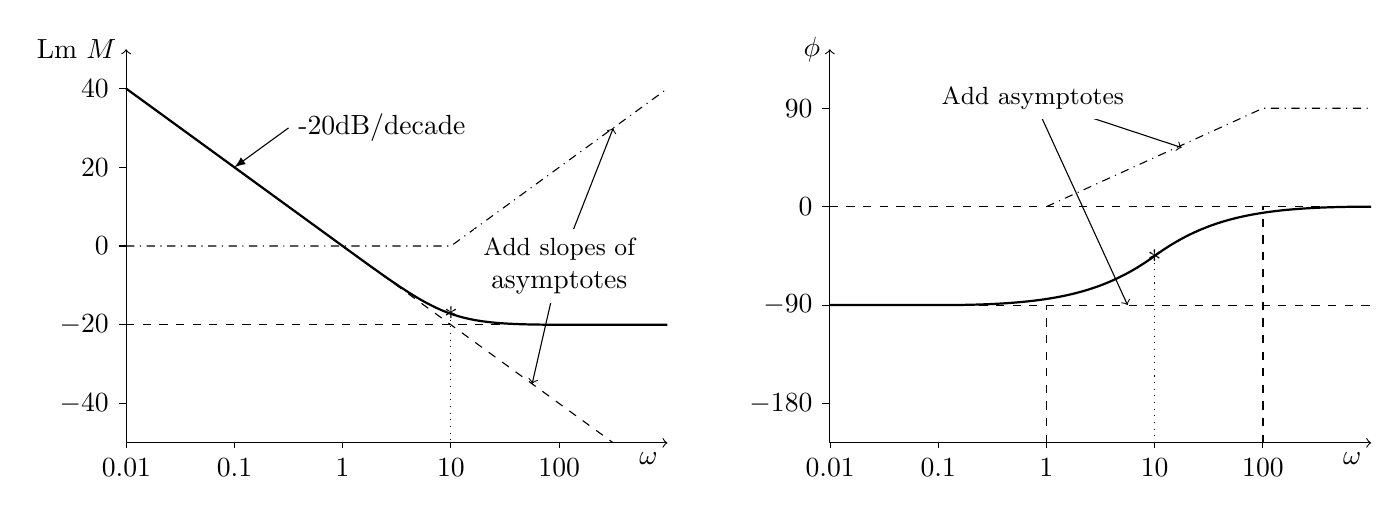
\begin{tikzpicture}[xscale=1.375]
		\draw[<->] (0,5) node[left] {$\Lm M$} |- (5,0) node[below left] {$ \omega $};
		
		\foreach \x [evaluate=\x as \xeval using log10(\x)+2] in {0.01,0.1,1,10,100} \draw (\xeval cm,0pt) -- (\xeval cm,-2pt) node[anchor=north] {$\x$};
		
		\foreach \y [evaluate=\y as \yeval using (\y+50)/20] in {40,20,0,-20,-40} \draw (0pt,\yeval cm) -- (-2pt,\yeval cm) node[anchor=east] {$\y$};
		
		\draw[dashed] (0,1.5) -- (5,1.5);
		\draw[dashed] (0,4.5) -- (4.5,0);
		\draw[dash dot] (0,2.5) -- (3,2.5) -- (5,4.5);
		\draw[dotted] (3,1.65) node {$ * $} -- (3,0);
		\draw[thick] (0,4.5) -- (2,2.5) ..controls (3,1.5) .. (4.25,1.5) -- (5,1.5);
		\draw[-latex] (1.5,4) node[right] {-20dB/decade} -- (1,3.5);
		\draw[<->] (3.75,0.75) -- (4,2.25) node[align=center,fill=white] {\small Add slopes of\\asymptotes} -- (4.5,4);
		
		\draw[xshift=6.5cm,<->] (0,5) node[left] {$\phi$} |- (5,0) node[below left] {$ \omega $};
		
		\foreach \x [evaluate=\x as \xeval using log10(\x)+2] in {0.01,0.1,1,10,100} \draw[xshift=6.5cm] (\xeval cm,0pt) -- (\xeval cm,-2pt) node[anchor=north] {$\x$};
		
		\foreach \y [evaluate=\y as \yeval using 1.25*(\y+180)/90+0.5] in {90,0,-90,-180} \draw[xshift=6.5cm] (0pt,\yeval cm) -- (-2pt,\yeval cm) node[anchor=east] {$\y$};
		
		\draw[thick,xshift=6.5cm] (0,1.75) -- (1,1.75) ..controls (2,1.75) and (2.5,1.875) .. (3,2.375) ..controls (3.5,2.875) and (4,3) .. (5,3);
		\draw[dashed,xshift=6.5cm] (0,1.75) -- (5,1.75);
		\draw[dashed,xshift=6.5cm] (0,3) -- (5,3);
		\draw[dotted,xshift=6.5cm] (3,2.375) node {$ * $} -- (3,0);
		\draw[dashed,xshift=6.5cm] (2,0) -- (2,1.75);
		\draw[dashed,xshift=6.5cm] (4,0) -- (4,3);
		\draw[dash dot,xshift=6.5cm] (2,3) -- (4,4.25) -- (5,4.25);
		
		\draw[<->,xshift=6.5cm] (2.75,1.75) -- (1.875,4.37
		5) node[align=right,fill=white] {\small Add asymptotes} -- (3.25,3.75);
	\end{tikzpicture}
\end{center}

\begin{minipage}{0.49\textwidth}
	\centering
	\begin{itemize}
		\item Start with $ -20 $dB/decade slope from integrator
		\item At $ \omega = \frac{1}{\tau} = 10 $rad/s, add 20dB/decade slope (net: 0dB/decade)
	\end{itemize}
\end{minipage}
\hfill
\begin{minipage}{0.49\textwidth}
	\centering
	\begin{itemize}
		\item Start with $ -90^\circ $ phase from integrator
		\item Add $ 90^\circ $ phase centered on $ \omega = \frac{1}{\tau} = 10 $rad/s (as $ \omega\to\infty $: $ \phi=0^\circ $)
	\end{itemize}
\end{minipage}

\exmp
Draw the Bode diagram for
\[ G(s) = \frac{10s+1}{s/10+1} \]
\[ \Rightarrow G(s) = 1\cdot (10s+1) \cdot \left(\frac{1}{s/10+1}\right)  \]
\begin{center}
	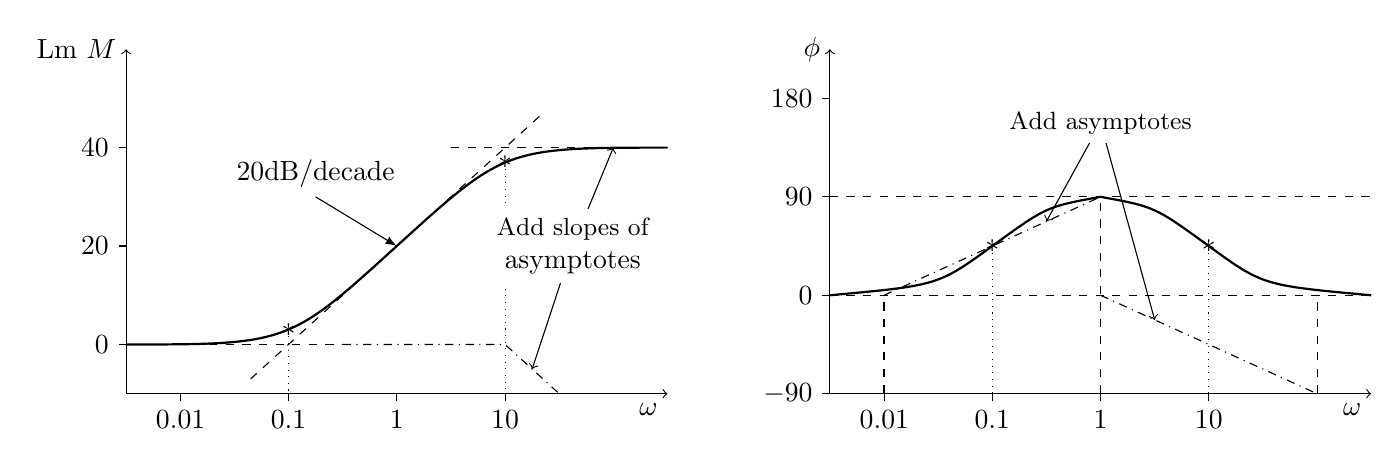
\begin{tikzpicture}[xscale=1.375,yscale=1.25]
	\draw[<->] (0,3.5) node[left] {$\Lm M$} |- (5,0) node[below left] {$ \omega $};
	
	\foreach \x [evaluate=\x as \xeval using log10(\x)+2.5] in {0.01,0.1,1,10} \draw (\xeval cm,0pt) -- (\xeval cm,-2pt) node[anchor=north] {$\x$};
	
	\foreach \y [evaluate=\y as \yeval using (\y+10)/20] in {40,20,0} \draw (0pt,\yeval cm) -- (-2pt,\yeval cm) node[anchor=east] {$\y$};
	
	\draw[dashed] (0,0.5) -- (2,0.5);
	\draw[dashed] (1.15,0.15) -- (3.85,2.85);
	\draw[dashed] (3,2.5) -- (5,2.5);
	\draw[dotted] (3.5,2.35) node {$ * $} -- (3.5,0);
	\draw[dotted] (1.5,0.65) node {$ * $} -- (1.5,0);
	\draw[thick] (0,0.5) ..controls (1.5,0.5) .. (2.5,1.5) ..controls (3.5,2.5) .. (5,2.5);
	\draw[-latex] (1.75,2) node[above] {20dB/decade} -- (2.5,1.5);
	\draw[dash dot] (2,0.5) -- (3.5,0.5) -- (4,0);
	\draw[<->] (3.75,0.25) -- (4.125,1.5) node[align=center,fill=white] {\small Add slopes of\\asymptotes} -- (4.5,2.5);
	
	\draw[xshift=6.5cm,<->] (0,3.5) node[left] {$\phi$} |- (5,0) node[below left] {$ \omega $};
	
	\foreach \x [evaluate=\x as \xeval using log10(\x)+2.5] in {0.01,0.1,1,10} \draw[xshift=6.5cm] (\xeval cm,0pt) -- (\xeval cm,-2pt) node[anchor=north] {$\x$};
	
	\foreach \y [evaluate=\y as \yeval using (\y+90)/90] in {90,0,-90,180} \draw[xshift=6.5cm] (0pt,\yeval cm) -- (-2pt,\yeval cm) node[anchor=east] {$\y$};
	
	\draw[thick,xshift=6.5cm] (0,1) ..controls (1,1.1) .. (1.5,1.5) ..controls (2,1.9) .. (2.5,2) ..controls(3,1.9) .. (3.5,1.5) ..controls (4,1.1) .. (5,1);
	\draw[dashed,xshift=6.5cm] (0,1) -- (5,1);
	\draw[dashed,xshift=6.5cm] (0,2) -- (5,2);
	\draw[dotted,xshift=6.5cm] (3.5,1.5) node {$ * $} -- (3.5,0);
	\draw[dotted,xshift=6.5cm] (1.5,1.5) node {$ * $} -- (1.5,0);
	\draw[dashed,xshift=6.5cm] (2.5,0) -- (2.5,2);
	\draw[dashed,xshift=6.5cm] (0.5,0) -- (0.5,1);
	\draw[dashed,xshift=6.5cm] (4.5,0) -- (4.5,1);
	\draw[dash dot,xshift=6.5cm] (0.5,1) -- (2.5,2);
	\draw[dash dot,xshift=6.5cm] (2.5,1) -- (4.5,0);
	
	\draw[<->,xshift=6.5cm] (2,1.75) -- (2.5,2.75) node[align=center,fill=white] {\small Add asymptotes} -- (3,0.75);
	\end{tikzpicture}
\end{center}

\begin{minipage}{0.49\textwidth}
	\centering
	\begin{itemize}
		\item Start with $ K=1 $: $ \Lm M = 0 $ and 0dB/decade slope
		\item At $ \omega = \frac{1}{\tau_z} = 0.1 $rad/s, add 20dB/decade slope (net: 20dB/decade)
		\item At $ \omega = \frac{1}{\tau_p} = 10 $rad/s, subtract 20dB/decade slope (net: 0dB/decade)
	\end{itemize}
\end{minipage}
\hfill
\begin{minipage}{0.49\textwidth}
	\centering
	\begin{itemize}
		\item Start with $ K=1 $: $ 0^\circ $ phase
		\item Add $ 90^\circ $ phase centered on $ \omega = \frac{1}{\tau_z} = 0.1 $rad/s (net: $ \omega=90^\circ $)
		\item Subtract $ 90^\circ $ phase centered on $ \omega = \frac{1}{\tau_p} = 10 $rad/s (net: $ \omega=0^\circ $)
	\end{itemize}
\end{minipage}

\section*{Bode Plot Summary}
\begin{itemize}
	\item Use superposition to sketch more complex Bode plots
	\begin{itemize}
		\item $ \Lm M_{total} = \sum \Lm M_{components} $
		\item $ \phi_{total} = \sum \phi_{components} $
	\end{itemize}
	\item Poles and zeros only have an effect for frequencies greater than the pole or zero ($ \omega>p $ or $ \omega>z $)
	\item Zeros add $ 90^\circ $ of phase and add 20dB/decade of slope for $ \omega>z $
	\item Poles subtract $ 90^\circ $ of phase and subtract 20dB/decade of slope for $ \omega>p $
\end{itemize}

\section*{Find a transfer function from a Bode plot}
\begin{minipage}{0.49\textwidth}
	Given a Bode plot that is \textbf{known} to be 2nd-order, can we find the transfer function?
	\begin{enumerate}
		\item Find where the phase plot crosses $ 90^\circ $. This frequency is $ \omega_n $.
		\item Find the magnitude at $ \omega_n $. This is $ 1/(2\zeta) $. 
	\end{enumerate}
	With $ \zeta $ and $ \omega_n $ known, the transfer function can be constructed.
\end{minipage}
\hfill
\begin{minipage}{\textwidth}
	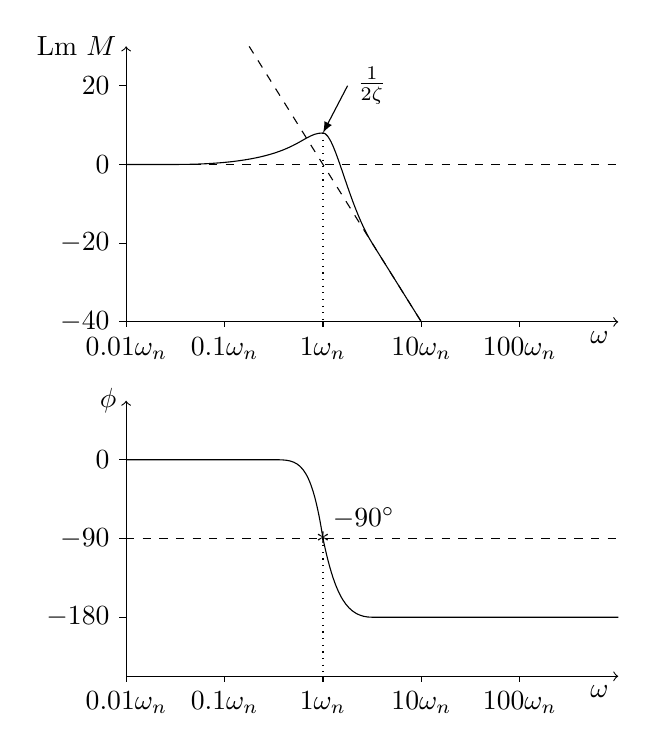
\begin{tikzpicture}[xscale=1.25]
		\draw[<->] (0,3.5) node[left] {$\Lm M$} |- (5,0) node[below left] {$ \omega $};
		
		\foreach \x [evaluate=\x as \xeval using log10(\x)+2] in {0.01,0.1,1,10,100} \draw (\xeval cm,0pt) -- (\xeval cm,-2pt) node[anchor=north] {${\x\omega_n}$};
		
		\foreach \y [evaluate=\y as \yeval using (\y+40)/20] in {-40,20,0,-20} \draw (0pt,\yeval cm) -- (-2pt,\yeval cm) node[anchor=east] {$\y$};
		
		\draw[dashed] (0,2) -- (5,2);
		\draw[dashed] (1.25,3.5) -- (3,0);
		\draw[dotted] (2,2.4) -- (2,0);
		%			\draw (0,2) -- (1,2) ..controls (2,2) .. (2.5,1) -- (3,0);
		%			\draw (0,2) -- (0.5,2) ..controls (1.75,2) and (1.75,2.2) .. (2,2.2) ..controls (2.125,2.2) and (2.25,1.5) .. (2.5,1) -- (3,0);
		\draw (0,2) -- (0.5,2) ..controls (1.75,2) and (1.75,2.4) .. (2,2.4) ..controls (2.125,2.4) and (2.25,1.5) .. (2.5,1) -- (3,0);
		% \draw[-latex] (3,1.5) node[right] {-40dB/decade} -- (2.5,1);
		\draw[-latex] (2.25,3) node[right] {$ \frac{1}{2\zeta} $} -- (2,2.4);
		%			\draw[-latex] (2.5,2.5) node[right] {$ \zeta=\frac{1}{2} $} -- (2,2.2);
		%			\draw[-latex] (1.75,1.25) node[left] {$ \zeta=\frac{1}{\sqrt{2}} $} -- (2,1.85);
		
		\draw[yshift=-4.5cm,<->] (0,3.5) node[left] {$\phi$} |- (5,0) node[below left] {$ \omega $};
		
		\foreach \x [evaluate=\x as \xeval using log10(\x)+2] in {0.01,0.1,1,10,100} \draw[yshift=-4.5cm] (\xeval cm,0pt) -- (\xeval cm,-2pt) node[anchor=north] {${\x\omega_n}$};
		
		\foreach \y [evaluate=\y as \yeval using (\y+180)/90+.75] in {-180,-90,0} \draw[yshift=-4.5cm] (0pt,\yeval cm) -- (-2pt,\yeval cm) node[anchor=east] {$\y$};
		
		%			\draw[yshift=-4.5cm] (0,2.75) ..controls (1,2.75) and (1.5,2.5) .. (2,1.75) ..controls (2.5,1) and (3,.75) .. (4,.75);
		%			\draw[yshift=-4.5cm] (0,2.75) -- (1,2.75) ..controls (1.5,2.75) and (1.75,2.5) .. (2,1.75) ..controls (2.25,1) and (2.5,.75) .. (3,.75) -- (4,.75);
		\draw[yshift=-4.5cm] (0,2.75) -- (1.5,2.75) ..controls (1.75,2.75) and (1.875,2.75) .. (2,1.75) ..controls (2.125,1) and (2.25,.75) .. (2.5,.75) -- (5,.75);
		\draw[dashed,yshift=-4.5cm] (0,1.75) -- (5,1.75);
		% \draw[dashed,yshift=-4.5cm] (0,2.75) -- (5,2.75);
		%	\draw[dashed,yshift=-4.5cm] (1,2.75) -- (3,0.75);
		%	\draw[dashed,yshift=-4.5cm] (1.5,2.75) -- (2.5,0.75);
		%	\draw[dashed,yshift=-4.5cm] (1.75,2.75) -- (2.25,0.75);
		%	\draw[dashed,yshift=-4.5cm] (1,0) -- (1,2);
		%	\draw[dashed,yshift=-4.5cm] (3,0) -- (3,1);
		\draw[dotted,yshift=-4.5cm] (2,1.75) node {$ * $} node[above right] {$ -90^\circ $} -- (2,0) ;
		%	\draw[-latex,yshift=-4.5cm] (1.6875,1.875) -- (2.0625,2.375) node[right] {Increasing $ \zeta $};
	\end{tikzpicture}
\end{minipage}

\clearpage

\section*{Feedback Principles}
Real systems have \textbf{disturbances} (uncontrolled inputs to the system).
\begin{center}
	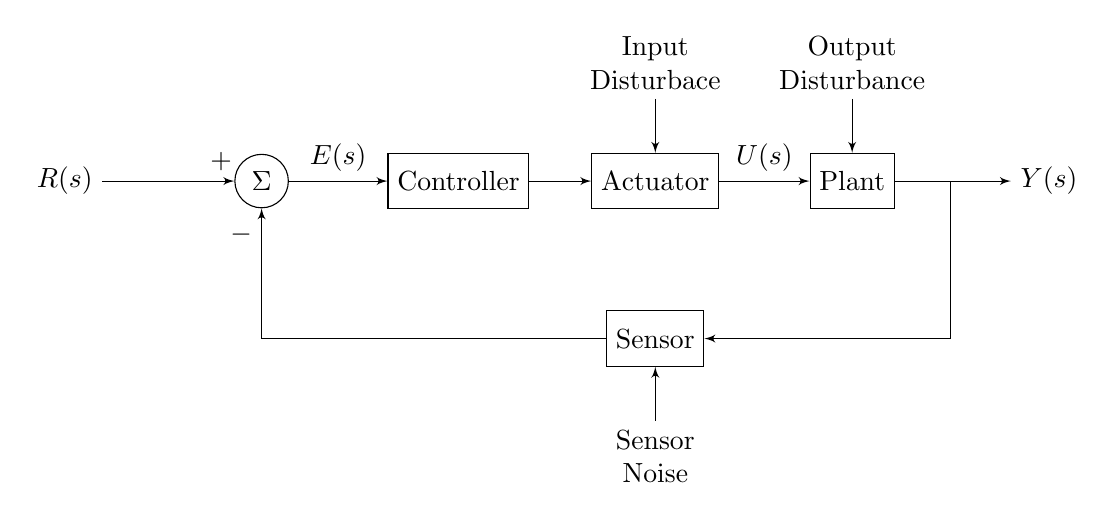
\begin{tikzpicture}[node distance=2.5cm,auto,>=latex']
		\node [input] (r) {$R(s)$};
		\node [sum] (sumr) [right of=r] {$\Sigma$};
		\node [block] (gc) [right of=sumr] {Controller};
		\node [block] (ga) [right of=gc] {Actuator};
		\node [block] (gp) [right of=ga] {Plant};
		\node [output] (y) [right of=gp]{$Y(s)$};
		\node [block] (h) [below of=ga,node distance=2cm] {Sensor};
		\node [input] (n) [below of=h,align=center,node distance=1.5cm]{Sensor\\Noise};
		\node [input] (dy) [above of=gp,node distance=1.5cm,align=center]{Output\\Disturbance};
		\node [input] (du) [above of=ga,node distance=1.5cm,align=center]{Input\\Disturbace};
		
		\draw[->] (r) -- node[pos=0.9] {$+$} (sumr);
		\draw[->] (sumr) -- node {$E(s)$} (gc);
		\draw[->] (gc) -- (ga);
		\draw[->] (ga) -- node {$U(s)$} (gp);
		\draw[->] (gp) -- (y);
		\draw[->] ($ (y)!0.5!(gp) $) |- (h);
		\draw[->] (n) -- (h);
		\draw[->] (h) -| node[pos=0.9] {$-$} (sumr);
		\draw[->] (du) -- (ga);
		\draw[->] (dy) -- (gp);
	\end{tikzpicture}
\end{center}
Modeled in conventional block diagram form,
\begin{center}
	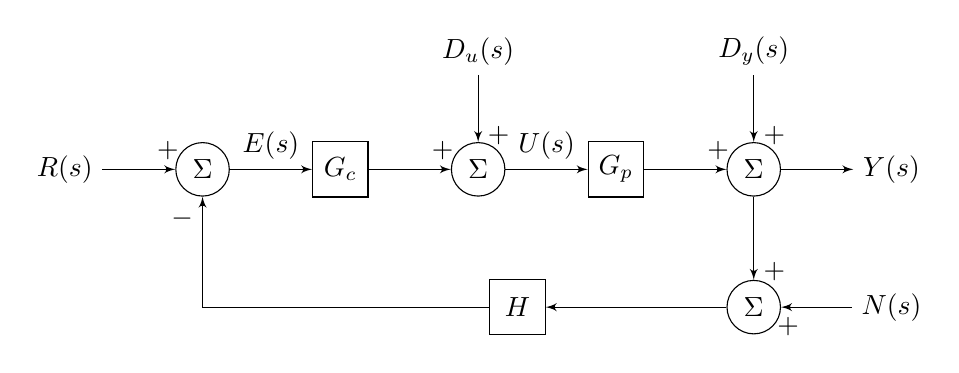
\begin{tikzpicture}[node distance=1.75cm,auto,>=latex']
	\node [input] (r) {$R(s)$};
	\node [sum] (sumr) [right of=r] {$\Sigma$};
	\node [block] (gc) [right of=sumr] {$ G_c $};
	\node [sum] (sumu) [right of=gc] {$\Sigma$};
	\node [block] (gp) [right of=sumu] {$ G_p $};
	\node [sum] (sumy) [right of=gp] {$\Sigma$};
	\node [output] (y) [right of=sumy]{$Y(s)$};
	\node [sum] (sumn) [below of=sumy] {$\Sigma$};
	\node [input] (n) [right of=sumn,align=center]{$ N(s) $};
	\node [block] (h) [left of=sumn,node distance=3cm] {$ H $};
	\node [input] (dy) [above of=sumy,node distance=1.5cm]{$ D_y(s) $};
	\node [input] (du) [above of=sumu,node distance=1.5cm]{$ D_u(s) $};
	
	\draw[->] (r) -- node[pos=0.9] {$+$} (sumr);
	\draw[->] (sumr) -- node {$E(s)$} (gc);
	\draw[->] (gc) -- node[pos=0.9] {$+$} (sumu);
	\draw[->] (du) -- node[pos=0.9] {$+$} (sumu);
	\draw[->] (sumu) -- node {$U(s)$} (gp);
	\draw[->] (gp) -- node[pos=0.9] {$+$} (sumy);		
	\draw[->] (dy) -- node[pos=0.9] {$+$} (sumy);
	\draw[->] (sumy) -- (y);
	\draw[->] (sumy) -- node[pos=0.9] {$+$} (sumn);
	\draw[->] (n) -- node[pos=0.9] {$+$} (sumn);
	\draw[->] (sumn) -- (h);
	\draw[->] (h) -| node[pos=0.9] {$-$} (sumr);
	\end{tikzpicture}
\end{center}
\noindent Typically:
\begin{itemize}
	\item $ G_p $ is known
	\item $ H $ is given
\end{itemize}
Goal: Design $ G_c $ such that
\begin{itemize}
	\item The feedback system is stable (internal stability)
	\item Transient behavior is good (minimal overshoot) --- time domain, performance metric
	\item Steady-state behavior is good (minimal steady-state error) --- time domain, performance metric
\end{itemize}
To simplify our closed-loop system, let's make some reasonable assumptions:
\begin{enumerate}
	\item Ignore $ D_u $ ($ D_u\approx0 $)
	\item $ H\approx1 $
\end{enumerate}
How do we justify these assumptions?
\begin{itemize}
	\item Typically, $ D_u \ll D_y $
	\item We may have some control over $ D_u $
	\item We want to use a sensor with negligible dynamics, otherwise it is not a good sensor.
\end{itemize}
So,
\begin{center}
	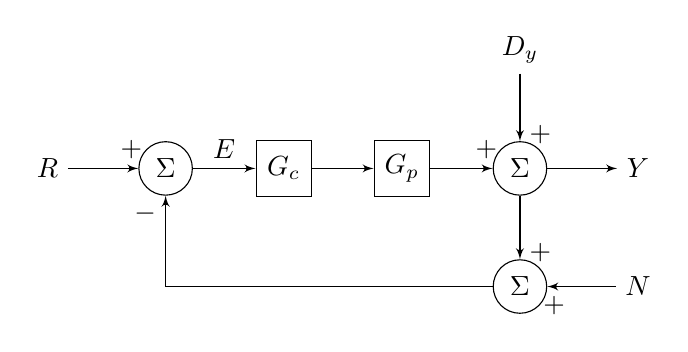
\begin{tikzpicture}[node distance=1.50cm,auto,>=latex']
	\node [input] (r) {$R$};
	\node [sum] (sumr) [right of=r] {$\Sigma$};
	\node [block] (gc) [right of=sumr] {$ G_c $};
	\node [block] (gp) [right of=gc] {$ G_p $};
	\node [sum] (sumy) [right of=gp] {$\Sigma$};
	\node [output] (y) [right of=sumy]{$Y$};
	\node [sum] (sumn) [below of=sumy] {$\Sigma$};
	\node [input] (n) [right of=sumn,align=center]{$ N $};
	\node [input] (dy) [above of=sumy,node distance=1.5cm]{$ D_y $};
	
	\draw[->] (r) -- node[pos=0.9] {$+$} (sumr);
	\draw[->] (sumr) -- node {$E$} (gc);
	\draw[->] (gc) -- (gp);
	\draw[->] (gp) -- node[pos=0.9] {$+$} (sumy);		
	\draw[->] (dy) -- node[pos=0.9] {$+$} (sumy);
	\draw[->] (sumy) -- (y);
	\draw[->] (sumy) -- node[pos=0.9] {$+$} (sumn);
	\draw[->] (n) -- node[pos=0.9] {$+$} (sumn);
	\draw[->] (sumn) -| node[pos=0.9] {$-$} (sumr);
	\end{tikzpicture}
\end{center}
\section*{Sensitivity and Complementary Sensitivity}
We will now introduce two new transfer functions used to describe the effect of disturbances on the system.

\textbf{Sensitivity} ($ S $) is the transfer function between the output disturbance $ D_y $ and the output $ Y $.
\[ \textrm{Sensitivity: } S = \frac{Y}{D_y} = \frac{1}{1+G_cG_p} \]

\textbf{Complementary Sensitivity} ($ T $) is the transfer function between the noise $ N $ and the output $ Y $.
\[ \textrm{Complementary Sensitivity: } T = \frac{Y}{N} = \frac{G_cG_p}{1+G_cG_p} \]

\section*{Controller Design}
When designing a controller, the disturbances present a challenge:
\begin{itemize}
	\item Input/Output disturbance
	\item Sensor noise
	\item Modeling error
	\item Variations in system parameters
\end{itemize}

\exmp
Consider a wind turbine where the controller goal is to maintain a constant rotational speed $ \Omega_R $ by controlling the blade pitch angle $ \beta $. What are some possible disturbances?
\begin{center}
	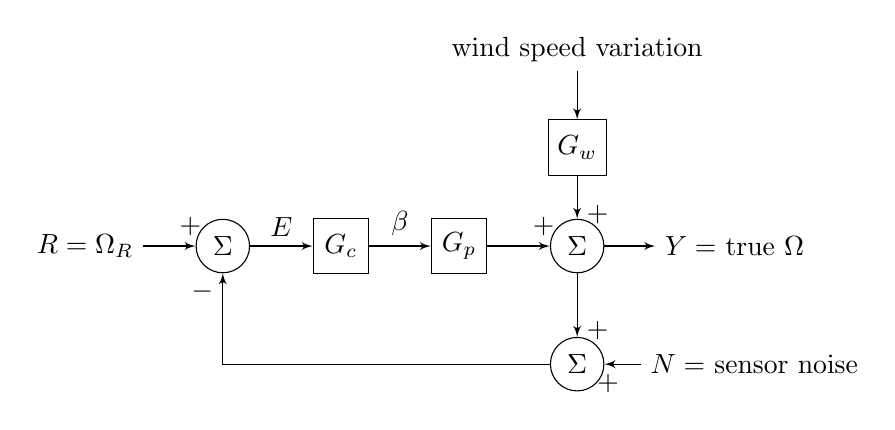
\begin{tikzpicture}[node distance=1.50cm,auto,>=latex']
	\node [input] (r) {$R=\Omega_R$};
	\node [sum] (sumr) [right of=r,node distance=1.75cm] {$\Sigma$};
	\node [block] (gc) [right of=sumr] {$ G_c $};
	\node [block] (gp) [right of=gc] {$ G_p $};
	\node [sum] (sumy) [right of=gp] {$\Sigma$};
	\node [output] (y) [right of=sumy,node distance=2cm]{$Y=$ true $ \Omega $};
	\node [sum] (sumn) [below of=sumy] {$\Sigma$};
	\node [input] (n) [right of=sumn,align=center,node distance=2.25cm]{$ N= $ sensor noise};
	\node [block] (gw) [above of=sumy,node distance=1.25cm] {$ G_w $};
	\node [input] (dy) [above of=gw,node distance=1.25cm]{wind speed variation};
	
	\draw[->] (r) -- node[pos=0.9] {$+$} (sumr);
	\draw[->] (sumr) -- node {$E$} (gc);
	\draw[->] (gc) -- node[above] {$ \beta $} (gp);
	\draw[->] (gp) -- node[pos=0.9] {$+$} (sumy);	
	\draw[->] (dy) -- (gw);	
	\draw[->] (gw) -- node[pos=0.9] {$+$} (sumy);
	\draw[->] (sumy) -- (y);
	\draw[->] (sumy) -- node[pos=0.9] {$+$} (sumn);
	\draw[->] (n) -- node[pos=0.9] {$+$} (sumn);
	\draw[->] (sumn) -| node[pos=0.9] {$-$} (sumr);
	\end{tikzpicture}
\end{center}
The wind turbine is subject to output disturbances (the impact of wind speed variation on rotational speed), sensor noise, modeling error (real dynamics are nonlinearl, but $ G_p $ is modeled as a linear system when designing $ G_c $), and variations in system parameters (e.g. changes in air density will change the plant).

\clearpage

\noindent We want our system to have:
\begin{itemize}
	\item Disturbance rejection --- frequency domain, performance metric
	\item Noise attenuation --- frequency domain, performance metric
	\item Robustness --- frequency domain, performance \textbf{and} stability metric
\end{itemize}

\subsection*{Disturbance Rejection}
\[ \textrm{Sensitivity: } S = \frac{Y}{D_y} = \frac{1}{1+G_cG_p} \]
If we don't want disturbances ($ D_y $) to have much effect on the output ($ Y $):
\begin{itemize}
	\item What do we want the magnitude of $ S $ to be? \textbf{Small.}
	\item What do we want the magnitude of $ G_cG_p $ to be for small $ S $? \textbf{Big.}
\end{itemize}

\begin{center}
	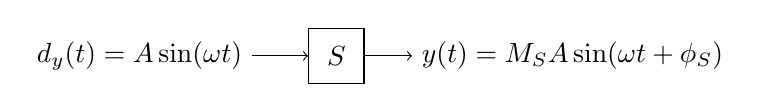
\begin{tikzpicture}[node distance = 2.5cm]
	\node[input] (in) {$ d_y(t)=A\sin(\wt) $};
	\node[block,right of=in] (sys) {$ S $};
	\node[output,right of=sys,node distance = 3cm] (out) {$ y(t)=M_SA\sin(\wt+\phi_S) $};
	\draw[->] (in)--(sys);
	\draw[->] (sys)--(out);
	\end{tikzpicture}
\end{center}
If $ M_S $ is small (magnitude of $ G_cG_p $ is large), then disturbances will be rejected at $ Y $.

\noindent Note: What is meant by ``small''?
\begin{itemize}
	\item Small compared to 1, i.e. $ M_S \ll 1 $.
	\item When $ M_S =1 $, the magnitude of the disturbance = the magnitude of the output.
\end{itemize}

\subsection*{Noise Attenuation}
\[ \textrm{Complementary Sensitivity: } T = \frac{Y}{N} = \frac{G_cG_p}{1+G_cG_p} \]
If we don't want disturbances ($ N $) to have much effect on the output ($ Y $):
\begin{itemize}
	\item What do we want the magnitude of $ T $ to be? \textbf{Small.}
	\item What do we want the magnitude of $ G_cG_p $ to be for small $ T $? \textbf{Small.}
\end{itemize}

\begin{center}
	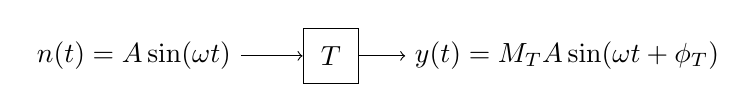
\begin{tikzpicture}[node distance = 2.5cm]
	\node[input] (in) {$ n(t)=A\sin(\wt) $};
	\node[block,right of=in] (sys) {$ T $};
	\node[output,right of=sys,node distance = 3cm] (out) {$ y(t)=M_TA\sin(\wt+\phi_T) $};
	\draw[->] (in)--(sys);
	\draw[->] (sys)--(out);
	\end{tikzpicture}
\end{center}
If $ M_T $ is small (magnitude of $ G_cG_p $ is small), then noise will be attenuated at $ Y $.

\noindent Note: What is meant by ``small''?
\begin{itemize}
	\item Small compared to 1, i.e. $ M_T \ll 1 $.
	\item But, $ \frac{Y}{R}=T $ and we want $ R=Y $. Therefore, $ M_T=1 $.
\end{itemize}

\subsection*{Loop Shaping}
We want both $ S $ and $ T $ to be small! Unfortunately, this isn't possible.
\[ \text{Small }G_cG_p \to \text{Small }T \]
\[ \text{Large }G_cG_p \to \text{Small }S \]
\[ S+T = \frac{1}{1+G_cG_p} + \frac{G_cG_p}{1+G_cG_p} \]
\[ \boxed{S+T=1} \]
If $ S $ and $ T $ add up to 1, can $ S $ or $ T $ be greater than 1? YES! $ S $ and $ T $ are complex numbers, so $ S+T=1 $ is like vector addition.

Improving disturbance rejection makes noise attenuation worse, and vice versa. What do we do?
\begin{itemize}
	\item What if I told you that disturbances are typically low-frequency signals and noise is a typically high-frequency signal?
	\begin{itemize}
		\item Make $ M_S\ll1 $ at low frequency
	
		($ M_T=1 $ at low frequency)
	
		\item Make $ M_T\ll1 $ at high frequency
		
		($ M_S=1 $ at high frequency)
	\end{itemize}
	\item In terms of $ G_cG_p $:
	\begin{itemize}
		\item Make $ G_cG_p $ large for low frequency and small for high frequency
	\end{itemize}
	\item A good shape for $ G_cG_p $ is something like:	
\end{itemize}

\begin{center}
	\begin{tikzpicture}[scale=2]
		\draw[<->] (0,3.5) node[left] {$\Lm M$} |- (5,0) node[below left] {$ \omega $};
				
		\draw[dashed] (0,1.5) node[left] {0dB} -| (2.5,0) node[below] {$ \omega_c $};
		\draw[thick] (0,3)-- (0.78125,2.375) ..controls (1.5625,1.75) .. (2.5,1.5) ..controls (3.4375,1.25) .. (4.21875,.625) -- (5,0);
		\node at (0.78125,2.375) {\begin{tikzpicture} \draw[dashed,rotate=-40] (0,0) ellipse (2.5 and 0.5); \end{tikzpicture}};
		\node at (2.5,1.5) {\begin{tikzpicture}\draw[dashed,rotate=-15] (0,0) ellipse (2 and 0.5);\end{tikzpicture}};
		\node at (4.21875,.625) {\begin{tikzpicture} \draw[dashed,rotate=-40] (0,0) ellipse (2.5 and 0.5); \end{tikzpicture}};
		
		\draw[-latex] (1.5,3) node[right,align=left] {Good disturbance\\rejection.} -- (1,2.5625);
		\draw[-latex] (3,2.375) node[right,align=left] {Determines robustness\\and stability.} -- (2.6875,1.6875);
		\draw[-latex] (4.375,1.5) node[above,align=center] {Good noise\\attenuation.} -- (4.1875,1);
	\end{tikzpicture}
\end{center}

\clearpage
\section*{Stability Revisited}
\begin{center}
	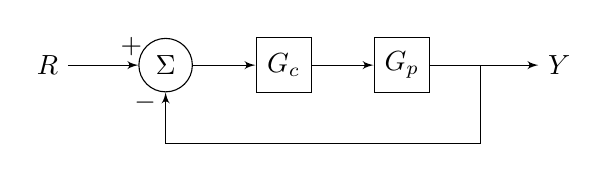
\begin{tikzpicture}[node distance=1.50cm,auto,>=latex']
		\node [input] (r) {$R$};
		\node [sum] (sumr) [right of=r] {$\Sigma$};
		\node [block] (gc) [right of=sumr] {$ G_c $};
		\node [block] (gp) [right of=gc] {$ G_p $};
		\node [output] (y) [right of=gp,node distance=2cm]{$Y$};
		\node [waypoint] (wp) [below of=gp,node distance=1cm] {};
		
		\draw[->] (r) -- node[pos=0.9] {$+$} (sumr);
		\draw[->] (sumr) -- (gc);
		\draw[->] (gc) --  (gp);
		\draw[->] (gp) -- (y);
		\draw[->] ($ (gp)!0.5!(y) $) |- (wp)-| node[pos=0.9] {$-$} (sumr);
	\end{tikzpicture}
\end{center}
\begin{itemize}
	\item The definition of stability relies on the location of the closed-loop poles:
	\[ den = 1+G_cG_p = 0 \quad \left(\text{where $ \dfrac{Y}{R}=\dfrac{num}{den} $}\right) \]
	\item But, this might not tell the entire story. There might be ``hidden poles'' not captured by that equation.
	\item For instance, we can design $ G_c $ to cancel out poles of $ G_p $.
	\item Why do we care about these hidden poles?
	\begin{itemize}
		\item \textbf{Because they can resurface when we don't expect it.}
	\end{itemize}
\end{itemize}
\exmp
\begin{center}
	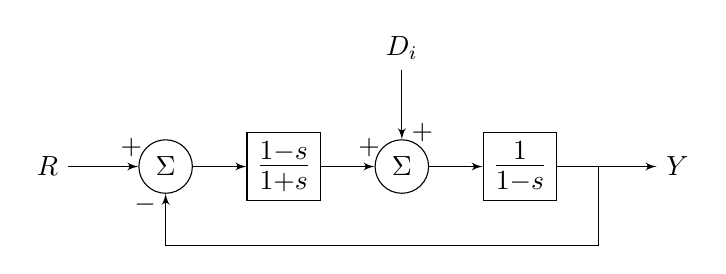
\begin{tikzpicture}[node distance=1.50cm,auto,>=latex']
	\node [input] (r) {$R$};
	\node [sum] (sumr) [right of=r] {$\Sigma$};
	\node [block] (gc) [right of=sumr] {\Large$\frac{1-s}{1+s}$};
	\node [sum] (sumu) [right of=gc] {$ \Sigma $};
	\node [input] (du) [above of=sumu] {$D_i$};
	\node [block] (gp) [right of=sumu] {\Large$\frac{1}{1-s}$};
	\node [output] (y) [right of=gp,node distance=2cm]{$Y$};
	\node [waypoint] (wp) [below of=gp,node distance=1cm] {};
	
	\draw[->] (r) -- node[pos=0.9] {$+$} (sumr);
	\draw[->] (sumr) -- (gc);
	\draw[->] (gc) -- node[pos=0.9] {$+$} (sumu);
	\draw[->] (du) -- node[pos=0.9] {$+$} (sumu);
	\draw[->] (sumu) -- (gp);	
	\draw[->] (gp) -- (y);
	\draw[->] ($ (gp)!0.5!(y) $) |- (wp)-| node[pos=0.9] {$-$} (sumr);
	\end{tikzpicture}
\end{center}
First, consider the closed-loop transfer function:
\[ \frac{Y}{R} = \frac{\frac{1-s}{1+s}\frac{1}{1-s}}{1+\frac{1-s}{1+s}\frac{1}{1-s}} = \frac{\frac{1}{s+1}}{1+\frac{1}{s+1}} = \frac{1}{s+2} \]
So, the closed-loop TF has a single, stable pole at $ s=-2 $. Now let's look at the effect of the input disturbance:
\[ \frac{Y}{D_i} = \frac{\frac{1}{1-s}}{1+\frac{1-s}{1+s}\frac{1}{1-s}} = \frac{\frac{s+1}{s-1}}{1+{s+1}} = \frac{s+1}{(s+2)(1-s)} \]
Even though the unstable pole was canceled out of the closed-loop TF, it is still present in the system's response to an input disturbance. 
\begin{itemize}
	\item We \textit{thought} we had a stable system, but the ``hidden'' pole came back to haunt us.
	\item A system is called \textbf{internally stable} if every closed-loop transfer function (not just $ R $ to $ Y $) is stable.
	\begin{itemize}
		\item This system is not internally stable.
	\end{itemize}
	\item In general, do not cancel unstable poles of the plant.
\end{itemize}


\end{document}